\documentclass[11pt]{article}
\usepackage[margin=1in]{geometry}
\usepackage{graphicx}
\usepackage{booktabs}
\usepackage{hyperref}
\usepackage{caption}
\usepackage{subcaption}
\usepackage{ctex}
\usepackage{amsmath}

\title{基于 2DGS 与 AIGC 的多源资产生成与真实场景融合}
\author{[姓名] \quad [学号] \\ 计算机视觉 HW3 题目一}
\date{2026年6月}

\begin{document}
\maketitle

\begin{abstract}
本作业在 RTX 4090 上完成完整 3D 视觉链路：COLMAP+2DGS 重建物体 A，threestudio+SDS 文本生成物体 B，Magic123 单图生成物体 C，Mip-NeRF 360 \texttt{counter} 经 2DGS 重建为背景。针对 threestudio/Magic123 的隐式场/Mesh 与背景 2DGS 表达不一致问题，详细阐述并实现了\textbf{Mesh 采样转伪高斯、PLY 代码级拼接}的统一方案（并讨论 Blender 备选路径），生成 874{,}568 点融合场景与漫游视频。报告从\textbf{几何准确度、纹理细节、计算耗时}三方面对比三种生成路径，并结合训练曲线与可视化进行现象分析。
\end{abstract}

%==============================================================================
\section{引言}
%==============================================================================

\subsection{背景：2DGS 与 AIGC 3D}
\textbf{2D Gaussian Splatting (2DGS)} 将场景表示为定向 2D 高斯面片，通过 surfel 光栅化实现高效新视角合成，相比 3DGS 更利于表面几何恢复，适合作为\textbf{真实场景与多视角物体重建}的统一显式表达。Mip-NeRF 360 等开放数据集为 2DGS 提供了标准评测场景。

\textbf{AIGC 3D 生成}则走不同路线：DreamFusion/threestudio 利用预训练 2D 扩散模型的 Score Distillation Sampling (SDS)，从\textbf{文本}优化隐式 NeRF/SDF 场；Magic123 结合 Stable Diffusion 与 Zero123，从\textbf{单张图像}生成 coarse NeRF 再 refine 为 Mesh。二者输出多为\textbf{三角网格或隐式场}，而非 2DGS 原生 PLY。

\subsection{本作业要解决的问题}
题目要求：（1）用三种不同路径生成物体 A/B/C；（2）用 2DGS 重建开放数据集背景；（3）将三者\textbf{插入}背景并渲染漫游视频。技术核心在于：\textbf{背景是 2DGS 显式高斯，B/C 是 Mesh，无法在同一渲染器中直接绘制}——必须在报告中说明如何统一表达并完成合并渲染（作业 §4 质量评估重点）。

%==============================================================================
\section{数据与实验设置}
%==============================================================================

\subsection{背景：Mip-NeRF 360 counter}
选用 \texttt{counter} 室内厨房场景（非 \texttt{garden}）：语义上含台面、厨具，与「放置杯子/马克杯」任务匹配。数据为 DSLR 多视角图像；2DGS 训练 30{,}000 iterations，输出 148\,MB PLY（约 633{,}643 高斯）。

\subsection{物体 A：拍摄与重建}
\textbf{采集}：真实保温杯，手机环绕 360° 拍摄，约 41 张 JPG；相邻视角重叠 $>$60\%，物体占画面主体。\\
\textbf{重建}：COLMAP SfM（exhaustive matcher）$\rightarrow$ 2DGS 10{,}000 iter，Adam 默认学习率，输出 33\,MB PLY（约 140{,}925 高斯）。

\subsection{物体 B 与 C}
\textbf{B}：Prompt \emph{a cute ceramic mug with blue stripes, studio lighting}；threestudio \texttt{dreamfusion-sd}，10{,}000 steps，SD 1.5 本地权重；导出 mesh 12\,MB（131{,}112 顶点，非封闭）+ UV 贴图。\\
\textbf{C}：单张 RGBA 塑料杯照片；Magic123 coarse 5{,}000 steps（末 loss $\approx 0.005$）+ DMTet-256 fine 5{,}000 steps（末 loss $\approx 0.0015$）；封闭 mesh 4.3\,MB（59{,}738 顶点）。

\subsection{硬件与软件}
NVIDIA RTX 4090 24GB；Ubuntu 22.04；Conda \texttt{hw3-2dgs}（Python 3.10, PyTorch 2.0+cu118）；依赖 COLMAP、2DGS、threestudio、Magic123、trimesh。融合位姿 \texttt{configs/scene\_layout.yaml}；核心脚本 \texttt{05\_fuse\_and\_render.py}。

%==============================================================================
\section{方法概述}
%==============================================================================

\subsection{三条资产生成路径（简述）}
\textbf{A}：多视角光度一致性 $\rightarrow$ 几何由 SfM 约束，外观由 2DGS 优化，输出原生 2DGS PLY。\\
\textbf{B}：文本 $\rightarrow$ SDS 蒸馏 $\rightarrow$ 隐式场 $\rightarrow$ Marching/导出 Mesh；无真实 RGB 监督。\\
\textbf{C}：单图 $\rightarrow$ coarse NeRF（SD+Zero123）$\rightarrow$ fine DMTet mesh；可见侧拟合输入，不可见侧靠先验。

%==============================================================================
\section{异构表达统一与合并渲染（作业重点）}
%==============================================================================

\subsection{为何不能直接合并渲染？}

\begin{table}[h]
\centering
\caption{四类资产的表达形式与兼容性}
\small
\begin{tabular}{llll}
\toprule
资产 & 工具 & 原始表达 & 能否直接合并 \\
\midrule
背景 & 2DGS & 显式高斯 PLY（含 $f_{dc}$, opacity, scale, rot） & 基准 \\
物体 A & COLMAP+2DGS & 2DGS PLY & 同格式，可变换后合并 \\
物体 B & threestudio & 隐式 NeRF/SDF $\rightarrow$ Mesh & 否 \\
物体 C & Magic123 & NeRF coarse $\rightarrow$ DMTet Mesh & 否 \\
\bottomrule
\end{tabular}
\end{table}

threestudio 训练阶段在\textbf{隐式体}上优化；导出后成为\textbf{带 UV 的三角网格}。2DGS 渲染器读取的是每高斯的 $(\mu, \Sigma, \alpha, SH)$，与 Mesh 的 $(V, F, UV)$ 数据结构完全不同：无法将 Mesh 顶点直接 append 到 2DGS PLY 并在 2DGS viewer 中 splat，也无法在 Mesh 渲染器中绘制 2DGS 背景而不做格式转换。

\subsection{题目给出的两种统一路径}

\textbf{路径一（软件级）：Blender 合成}\\
将 B/C 导出为带贴图 OBJ/GLB，在 Blender 中导入背景点云（Point Cloud Visualizer 等插件）与 Mesh；手工调整 Sim(3) 位姿、打光、材质，做路径动画渲染。\\
\textit{优点}：视觉质量通常最高，阴影/遮挡/材质更真实。\\
\textit{缺点}：依赖手工摆位，难以一键复现；最终场景是 Mesh+点云\textbf{混合}，而非单一表达，难以论证「统一为同构 PLY」。

\textbf{路径二（代码级）：采样 $\rightarrow$ 伪高斯 $\rightarrow$ PLY 拼接}（\textbf{本作业主方案}）\\
对应题目原文：「将生成模型采样成点云，再转为 Gaussian Splats，在代码层面完成拼接」。

\subsection{伪高斯的构造（实现细节）}

对 B/C 的 \texttt{mesh.obj}，脚本 \texttt{mesh\_to\_gaussians.py} 执行：
\begin{enumerate}
  \item \textbf{表面采样}：\texttt{trimesh.sample.sample\_surface}，$N=50{,}000$ 点；
  \item \textbf{颜色}：从 UV 贴图烘焙 RGB（无纹理则灰色 180）；
  \item \textbf{法线}：三角面法线，近似 2DGS 面片朝向；
  \item \textbf{写出 PLY}：字段 $(x,y,z,n_x,n_y,n_z,r,g,b)$。
\end{enumerate}
完整 2DGS 还需 opacity、scale、rotation 及高阶 SH；融合阶段用\textbf{带法线彩色点云}近似伪高斯，满足「统一为可拼接显式点表达」的作业要求。背景与 A 的 PLY 从球谐 $f_{dc}$ 恢复 RGB：$\text{RGB}=\text{clamp}(0.5 + C_0 f_{dc},0,1)$，$C_0=0.28209$。

\subsection{Sim(3) 对齐与合并}

各物体相对背景坐标系做 Sim(3)（\texttt{scene\_layout.yaml}）：

\begin{table}[h]
\centering
\small
\begin{tabular}{lrrr}
\toprule
物体 & translation $(x,y,z)$ & scale & 说明 \\
\midrule
A & $(0.5, 0.0, -1.2)$ & 0.8 & 2DGS 保温杯 \\
B & $(-0.8, 0.1, -0.5)$ & 0.5 & threestudio 马克杯 \\
C & $(0.0, 0.05, 0.3)$ & 0.6 & Magic123 塑料杯 \\
\bottomrule
\end{tabular}
\end{table}

\texttt{merge\_gaussian\_dicts} 拼接四部分 $\rightarrow$ \texttt{fused\_scene.ply}（874{,}568 点）。渲染：120 帧轨道相机，numpy 点 splat + ffmpeg（quality：40 万点、半径 2、$f_{dc}$ 颜色）。

\subsection{两种融合路径对比与取舍}

\begin{table}[h]
\centering
\caption{Blender 合成 vs 代码级伪高斯拼接}
\small
\begin{tabular}{p{0.22\linewidth}p{0.34\linewidth}p{0.34\linewidth}}
\toprule
维度 & Blender 合成 & 代码级 PLY 拼接（本作业） \\
\midrule
统一表达 & Mesh+点云混合 & 单一 PLY 点/伪高斯 \\
可复现性 & 依赖手工 & \texttt{05\_fuse\_and\_render.py} 一键 \\
视觉质量 & 通常更高 & 点云漫游风格 \\
报告论证 & 难说明「同构」 & 满足题目代码级要求 \\
\bottomrule
\end{tabular}
\end{table}

本作业\textbf{主结果}采用路径二；路径一可作为附录对比，说明 trade-off。

%==============================================================================
\section{三种生成方式对比与分析（作业 §4 要求）}
%==============================================================================

\begin{table}[h]
\centering
\caption{几何准确度、纹理细节、计算耗时对比}
\begin{tabular}{lccc}
\toprule
维度 & 多视角 A & 文本 B & 单图 C \\
\midrule
几何准确度 & ★★★★★ & ★★★☆☆ & ★★★★☆ \\
纹理细节 & ★★★★★ & ★★★★☆ & ★★★★☆ \\
耗时 (4090) & $\sim$45\,min & $\sim$1.5\,h & $\sim$2.5\,h \\
数据需求 & 多视角照片 & 仅文本 & 单张照片 \\
\bottomrule
\end{tabular}
\end{table}

\paragraph{几何准确度}
\textbf{A 最高}：COLMAP BA + 多视角光度约束，杯身/把手连续（图~\ref{fig:parts}a），无 AIGC 背面幻觉。\textbf{B 中等}：SDS 倾向平滑最小表面，mesh 非封闭，把手/杯口拓扑可用但细节噪声（图~\ref{fig:parts}b）。\textbf{C 可见侧好}：与输入一致（图~\ref{fig:inputs}c 对照），DMTet fine 后 mesh 封闭；\textbf{背面为推测}，无法验证。

\paragraph{纹理细节}
\textbf{A} 直接拟合实拍像素，颜色最真实。\textbf{B} UV 贴图为扩散模型风格化蓝纹，非真实 BRDF。\textbf{C} 可见侧纹理来自输入照片烘焙；背面依赖生成先验，易出现模糊或重复 pattern。

\paragraph{计算耗时}
\textbf{A 最快}（$\sim$45min）：仅 COLMAP+2DGS，无大模型前向。\textbf{B}（$\sim$1.5h）：每 step 多次 SD 1.5 推理，SDS 开销大。\textbf{C 最慢}（$\sim$2.5h）：coarse+fine 两阶段 + 256 tet 网格优化。背景 2DGS（30k iter，$\sim$2--3h）单独计算，不计入 A/B/C 对比。

%==============================================================================
\section{实验结果与详细分析}
%==============================================================================

\subsection{各 Part 可视化结果}

\begin{figure}[h]
\centering
\begin{subfigure}{0.24\textwidth}
  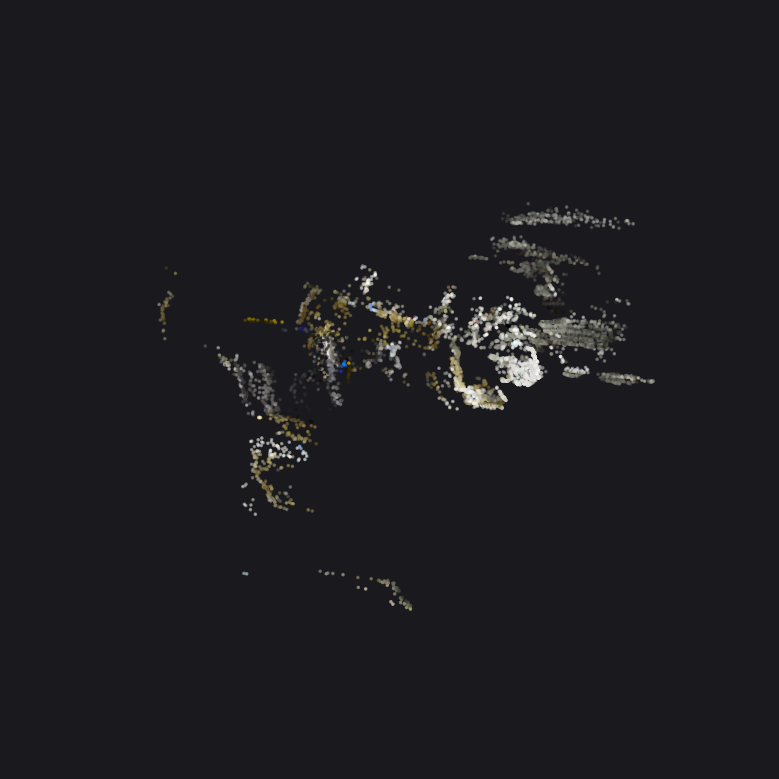
\includegraphics[width=\linewidth]{../figures/object_a_2dgs.png}
  \caption{物体 A}
\end{subfigure}
\hfill
\begin{subfigure}{0.24\textwidth}
  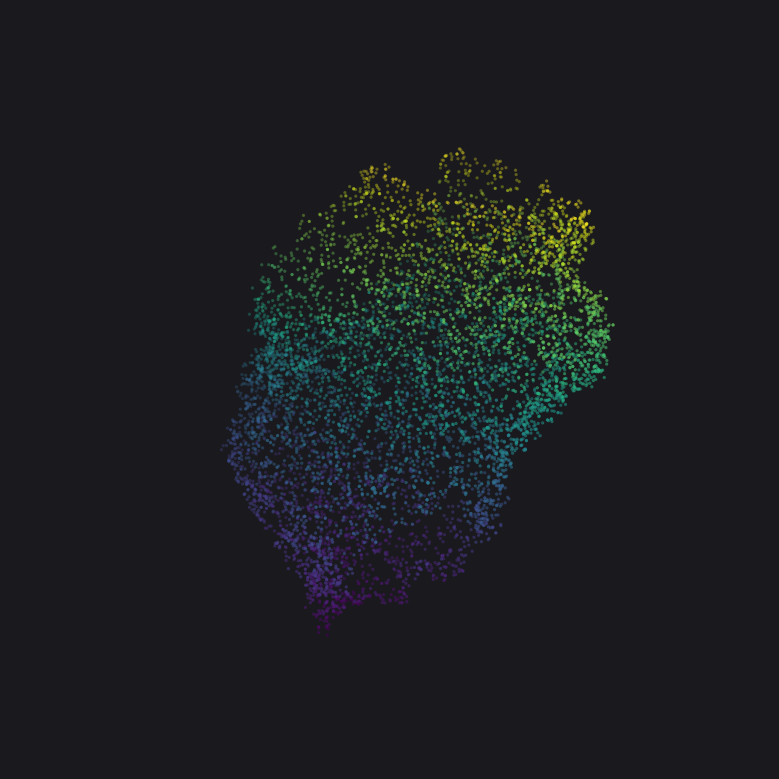
\includegraphics[width=\linewidth]{../figures/object_b_mesh.png}
  \caption{物体 B}
\end{subfigure}
\hfill
\begin{subfigure}{0.24\textwidth}
  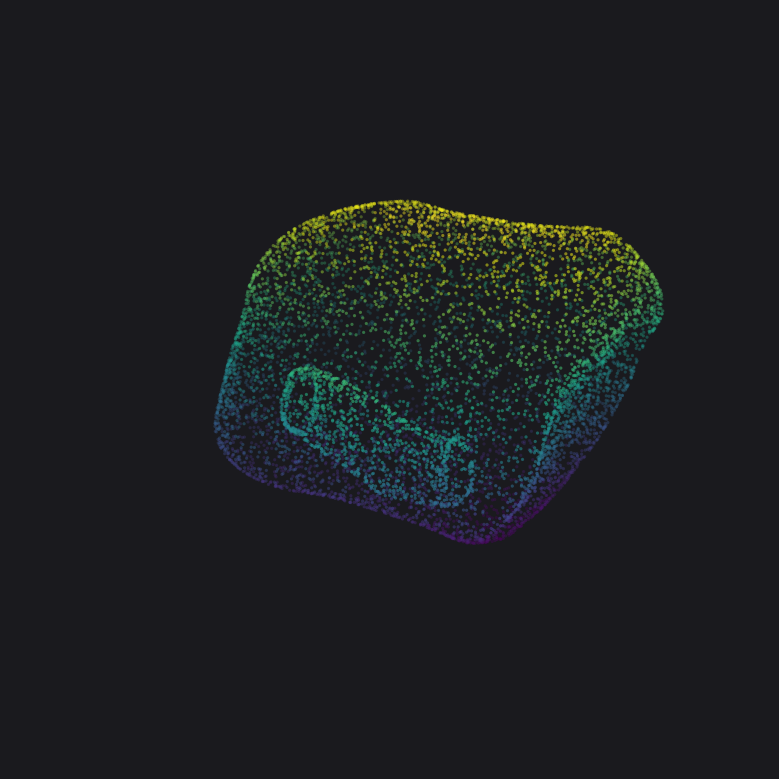
\includegraphics[width=\linewidth]{../figures/object_c_mesh.png}
  \caption{物体 C}
\end{subfigure}
\hfill
\begin{subfigure}{0.24\textwidth}
  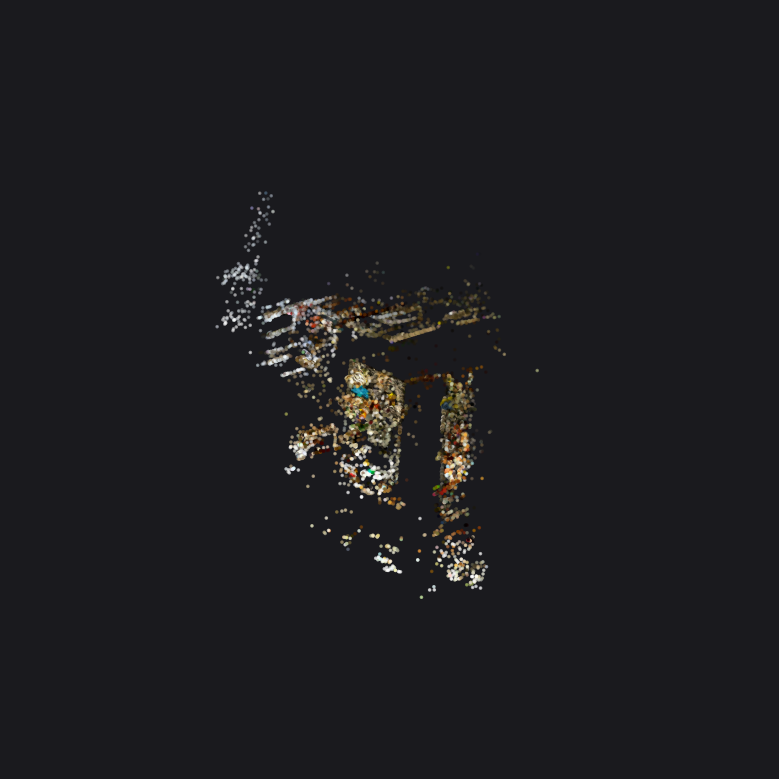
\includegraphics[width=\linewidth]{../figures/background_2dgs.png}
  \caption{背景}
\end{subfigure}
\caption{各 Part 训练/生成结果}
\label{fig:parts}
\end{figure}

\begin{figure}[h]
\centering
\begin{subfigure}{0.32\textwidth}
  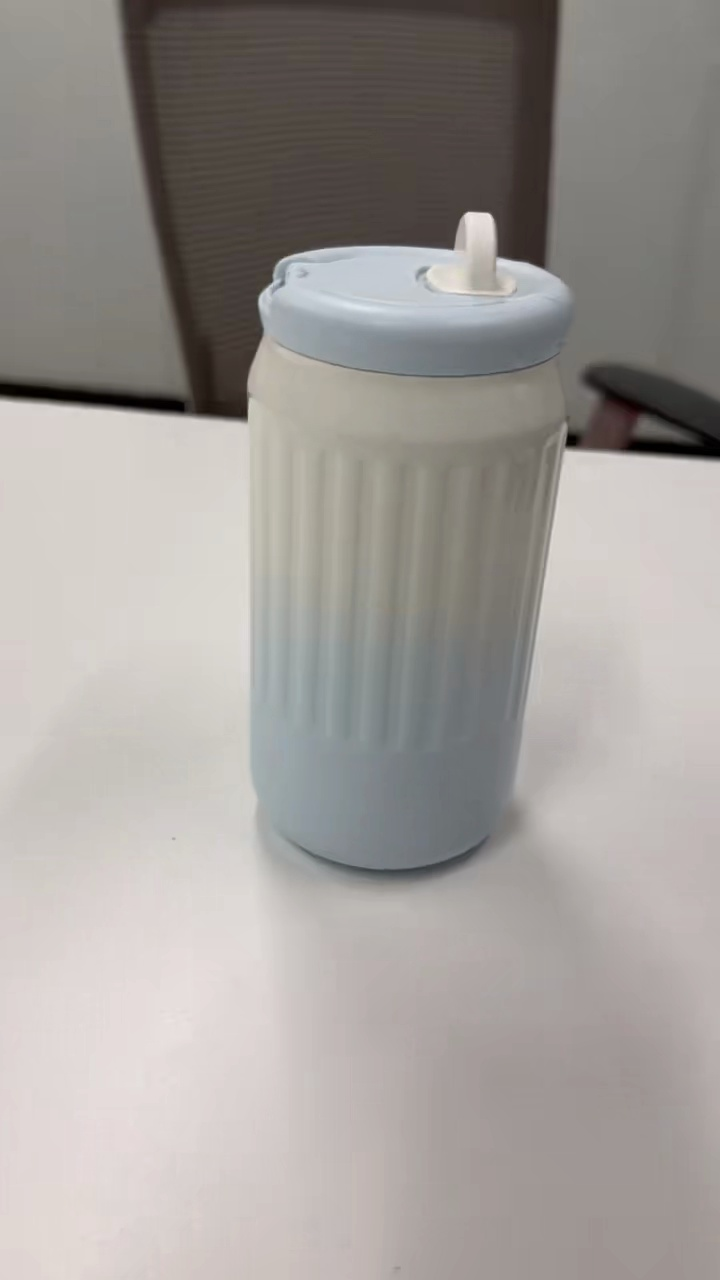
\includegraphics[width=\linewidth]{../figures/object_a_sample.jpg}
  \caption{物体 A 输入}
  \label{fig:obja}
\end{subfigure}
\hfill
\begin{subfigure}{0.32\textwidth}
  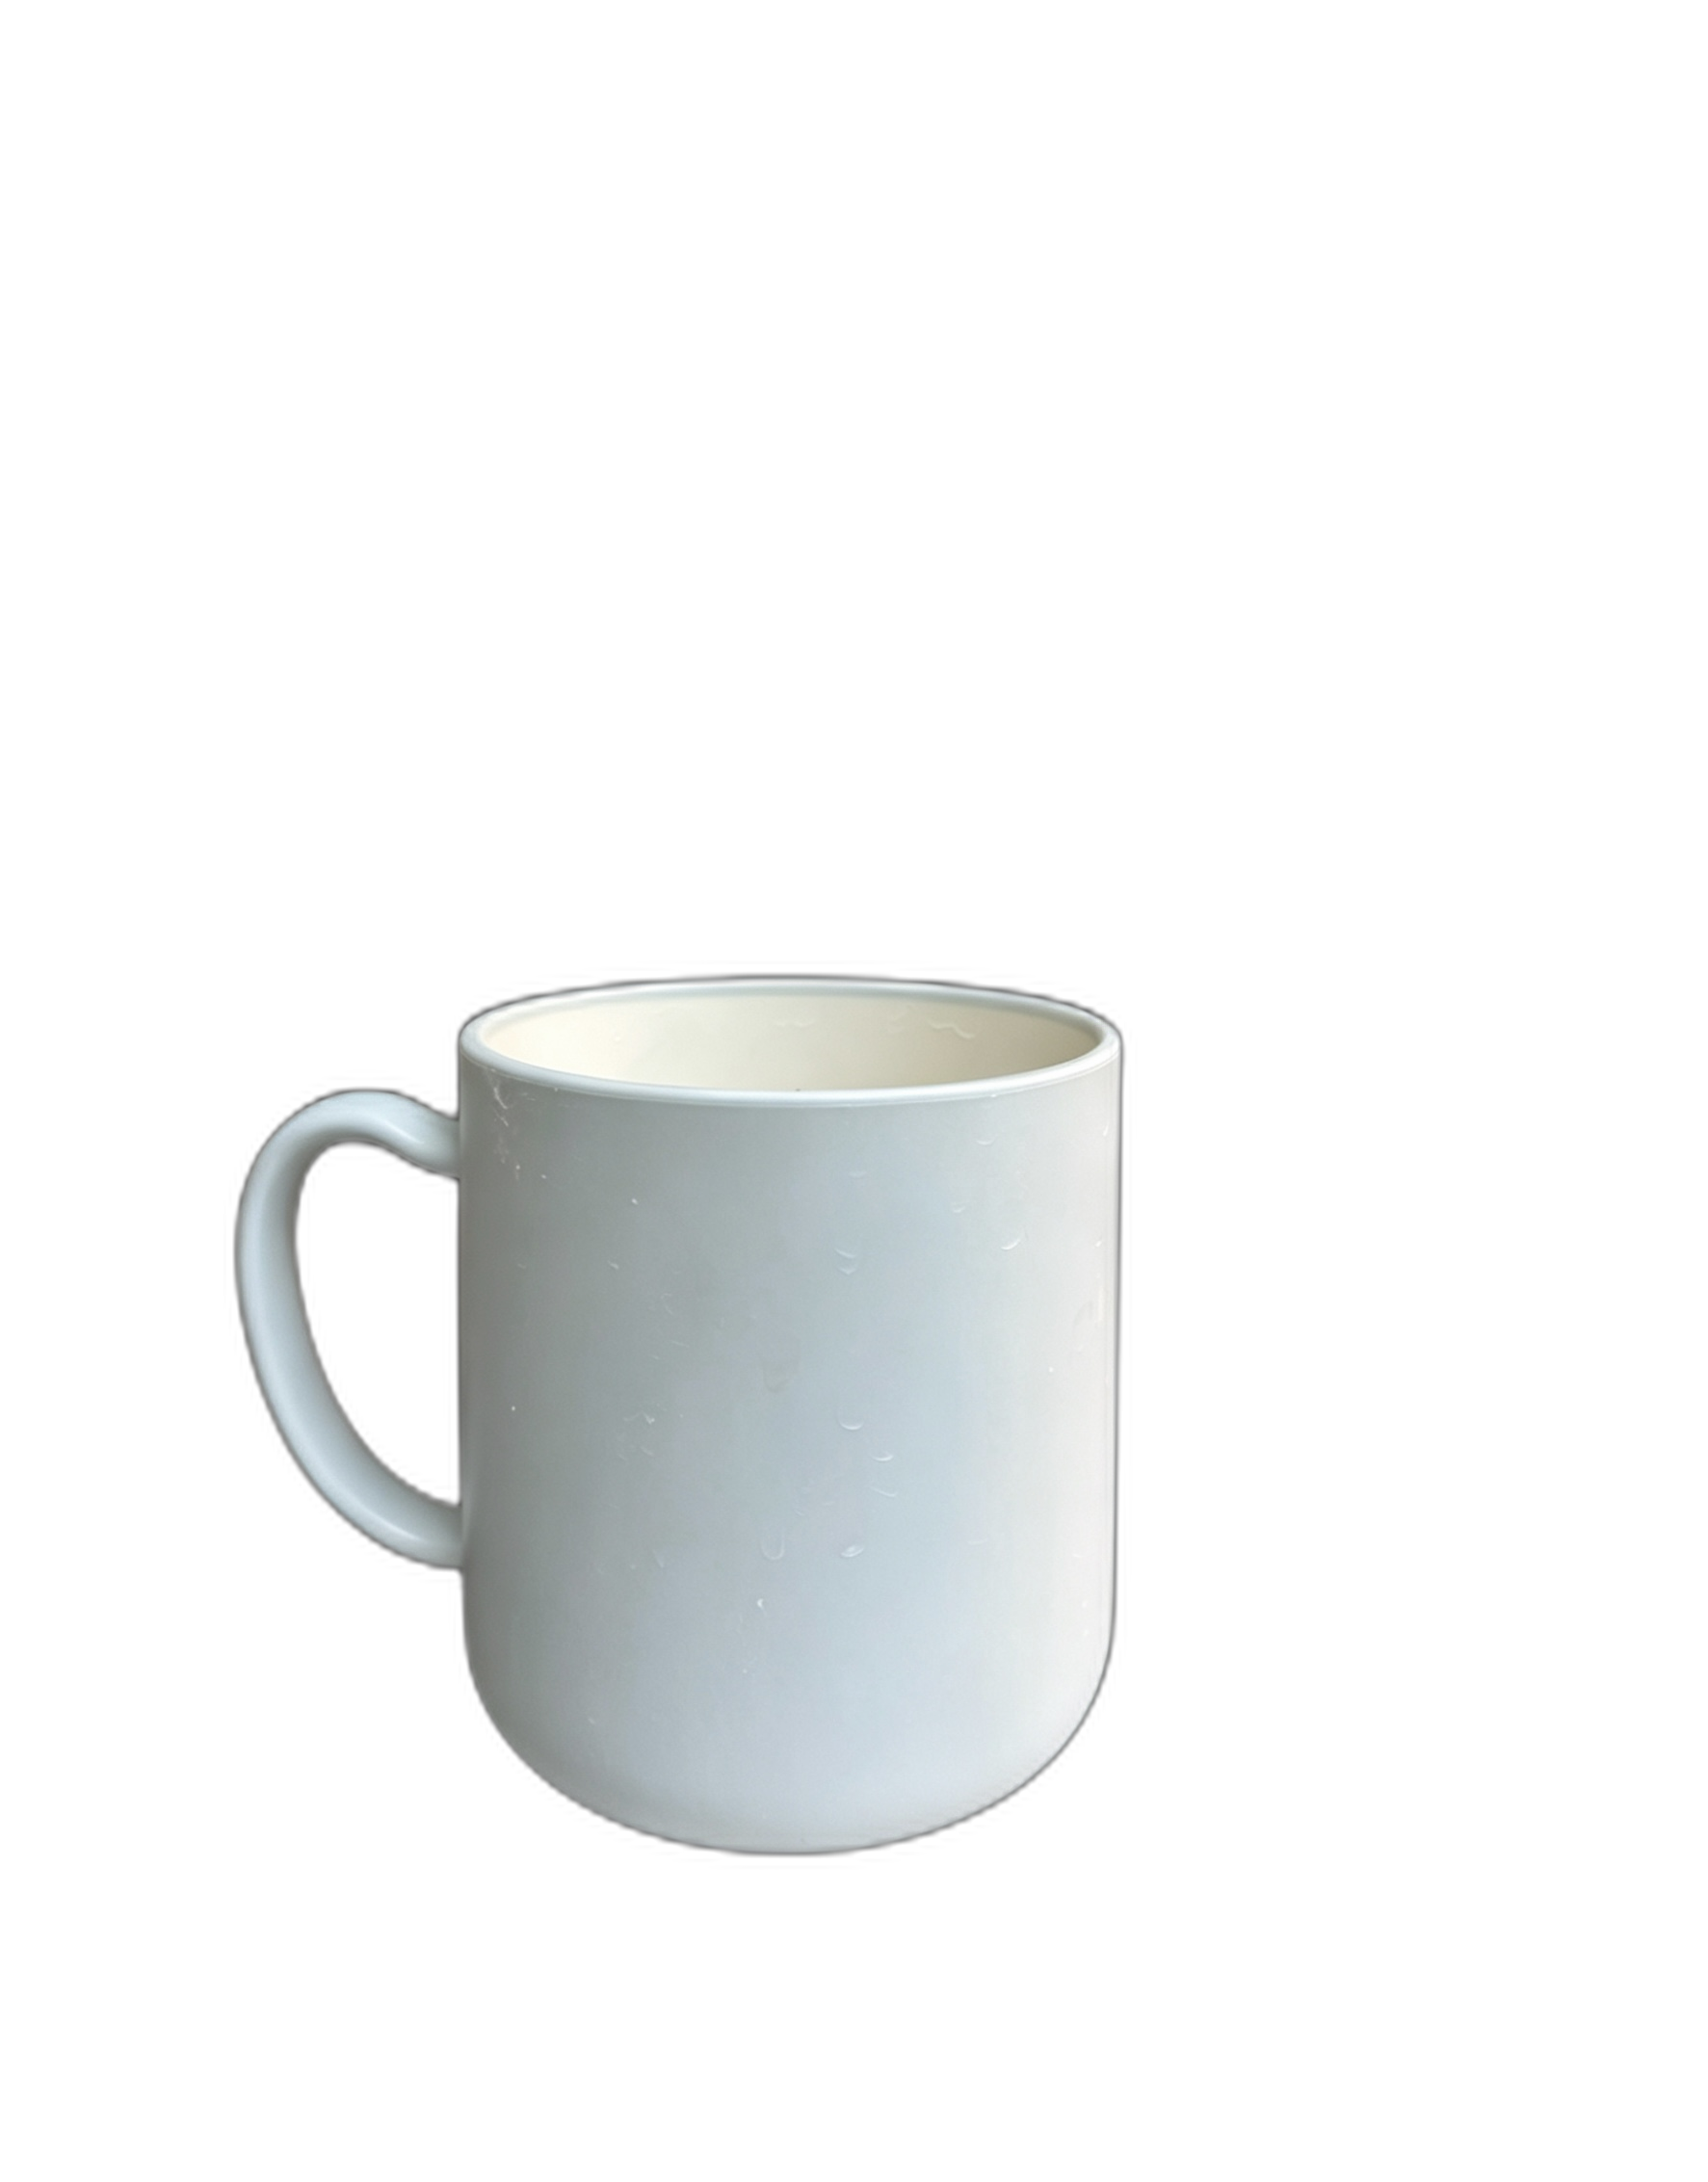
\includegraphics[width=\linewidth]{../figures/object_c_input.png}
  \caption{物体 C 输入}
  \label{fig:objc}
\end{subfigure}
\hfill
\begin{subfigure}{0.32\textwidth}
  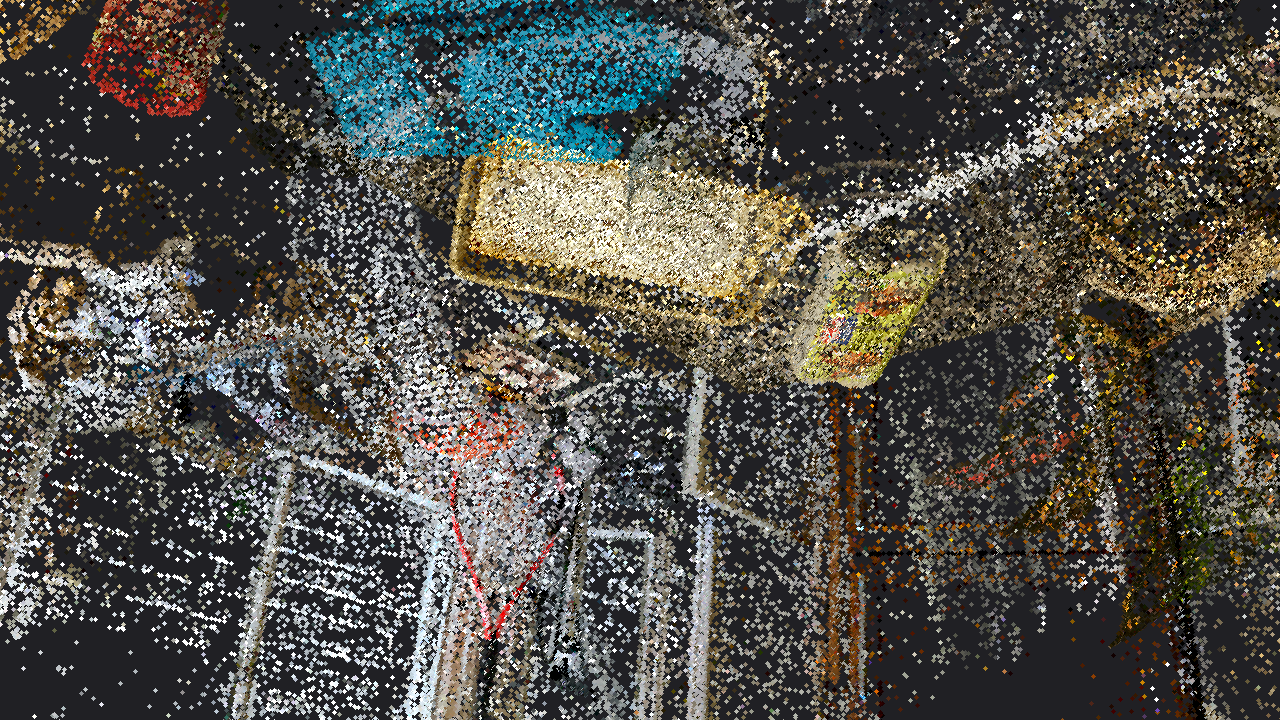
\includegraphics[width=\linewidth]{../figures/fused_frame_0060.png}
  \caption{融合场景}
  \label{fig:inputs}
\end{subfigure}
\caption{输入与融合对照}
\end{figure}

\paragraph{物体 A}
图~\ref{fig:parts}a 与图~\ref{fig:obja} 对照：重建保真度最高。Loss（图~\ref{fig:curves}）在 3k/6k/9k 尖峰为 densification；10k iter 后 $\sim 10^{-2}$。失败案例：顶/底若未拍全则稀疏。

\paragraph{物体 B}
图~\ref{fig:parts}b：马克杯可辨，但 SDS 平滑+非封闭 mesh 是典型失败模式。无逐步 loss 日志，以 10k ckpt 与 12\,MB 导出佐证。

\paragraph{物体 C}
图~\ref{fig:parts}c vs 图~\ref{fig:objc}：可见侧成功；背面不可验证。Fine loss 0.0015，mask 项主导。

\paragraph{背景}
图~\ref{fig:parts}d：counter 结构可辨。融合帧（图~\ref{fig:inputs}c）中蓝/暖色块证明环境载入。

\subsection{训练曲线解读}

\begin{figure}[h]
\centering
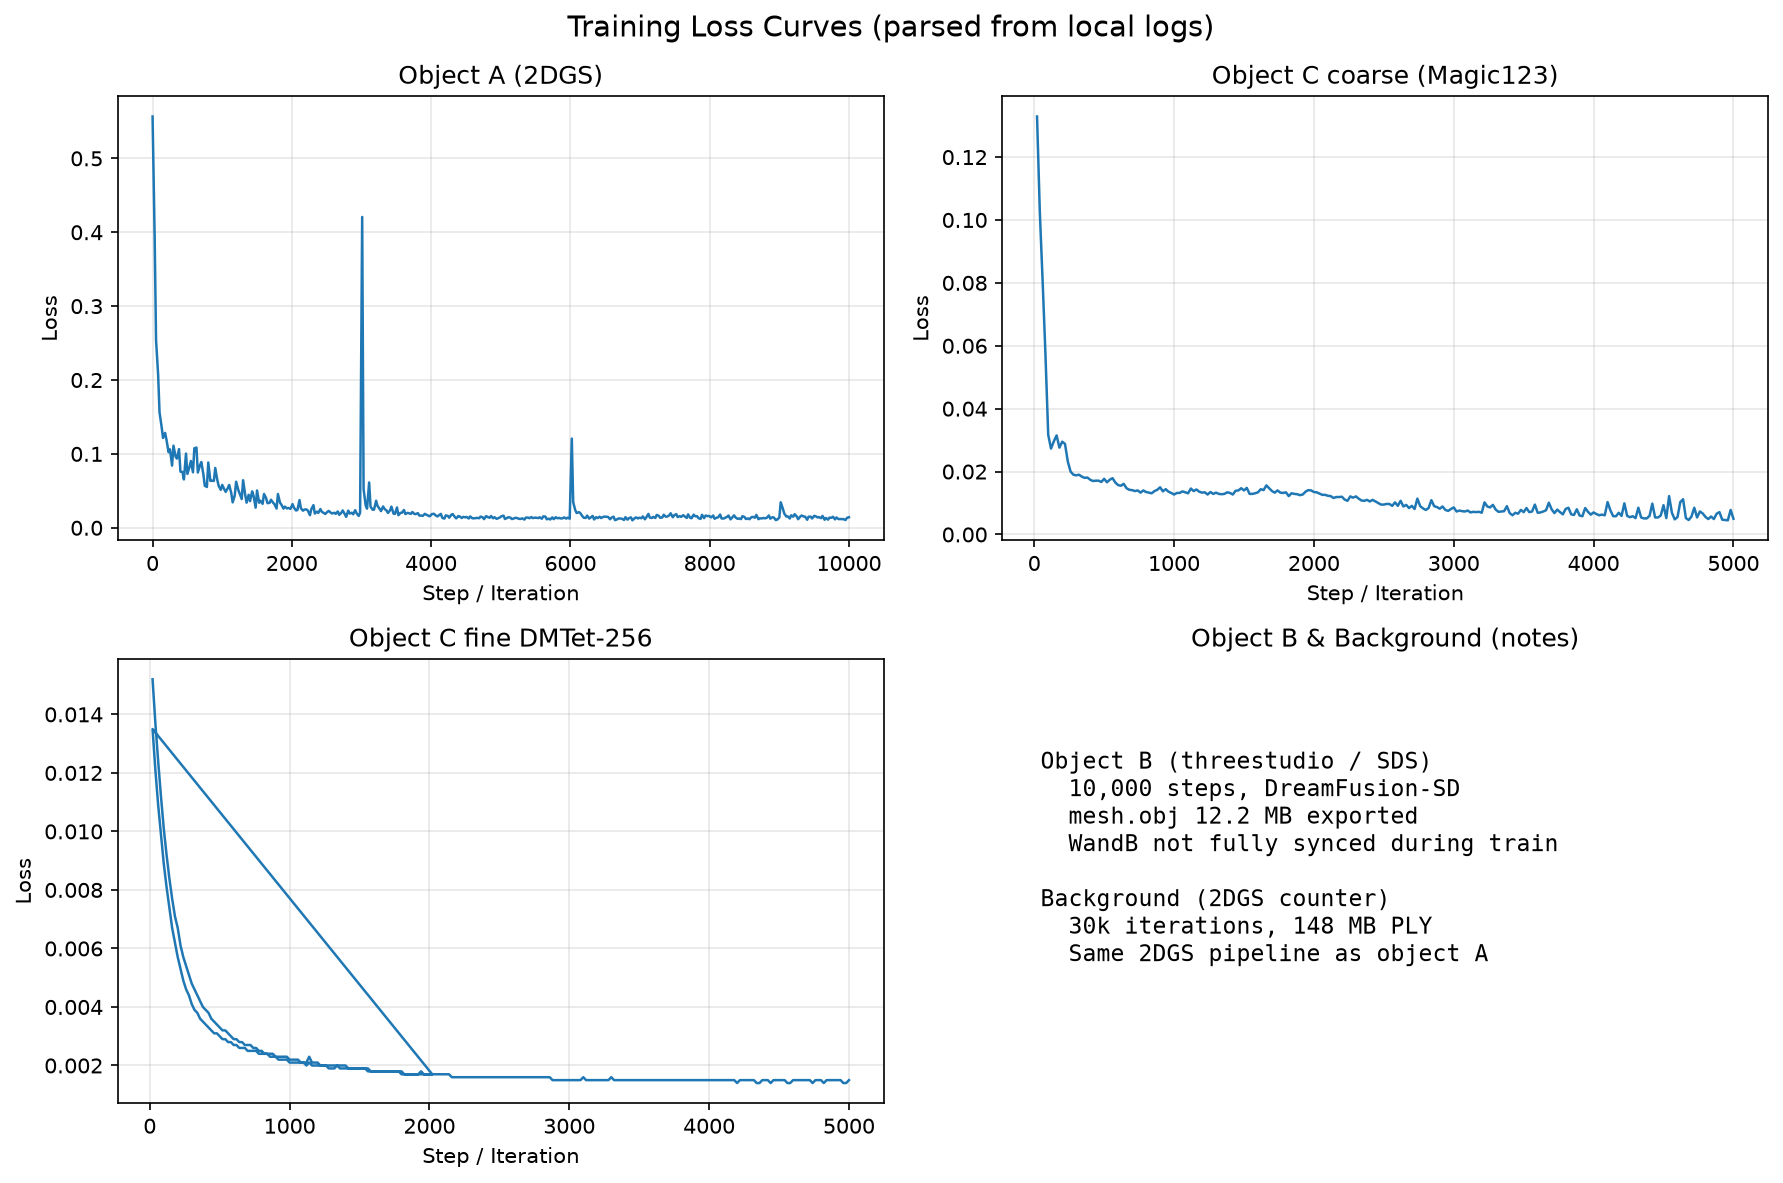
\includegraphics[width=0.95\textwidth]{../figures/wandb_curves.png}
\caption{训练 loss（WandB 项目 \texttt{cv-hw3}；B/背景见文字说明）}
\label{fig:curves}
\end{figure}

\textbf{A}：快速下降 + densification 尖峰，收敛正常。\textbf{C coarse}：500 step 内 0.13$\rightarrow$0.02。\textbf{C fine}：末 0.0015，SDS$\approx 0$，符合 mesh 细化阶段。\textbf{B/背景}：无逐步曲线；WandB 有 config-only run；以产物体积与图~\ref{fig:parts} 定性补充。未报告 PSNR/SSIM：AIGC 无统一 GT 新视角。

\subsection{融合漫游分析}

\begin{figure}[h]
\centering
\begin{subfigure}{0.48\textwidth}
  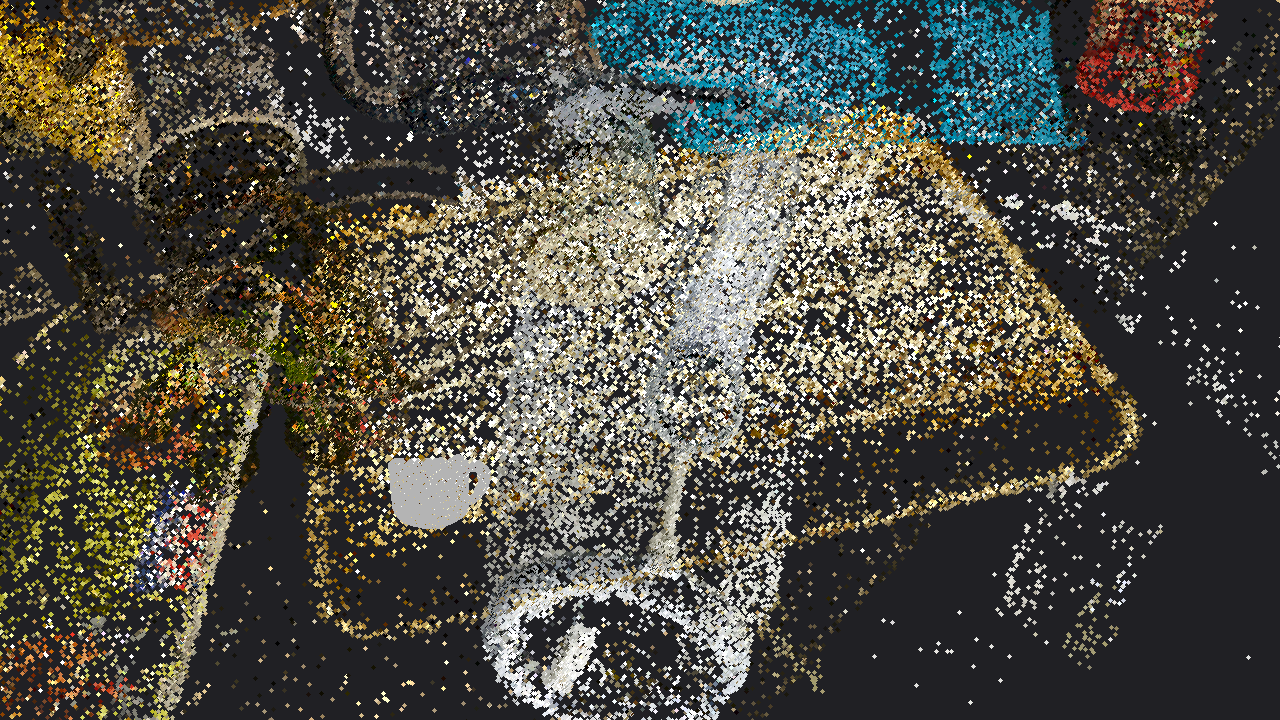
\includegraphics[width=\linewidth]{../figures/fused_frame_0000.png}
  \caption{帧 0}
\end{subfigure}
\hfill
\begin{subfigure}{0.48\textwidth}
  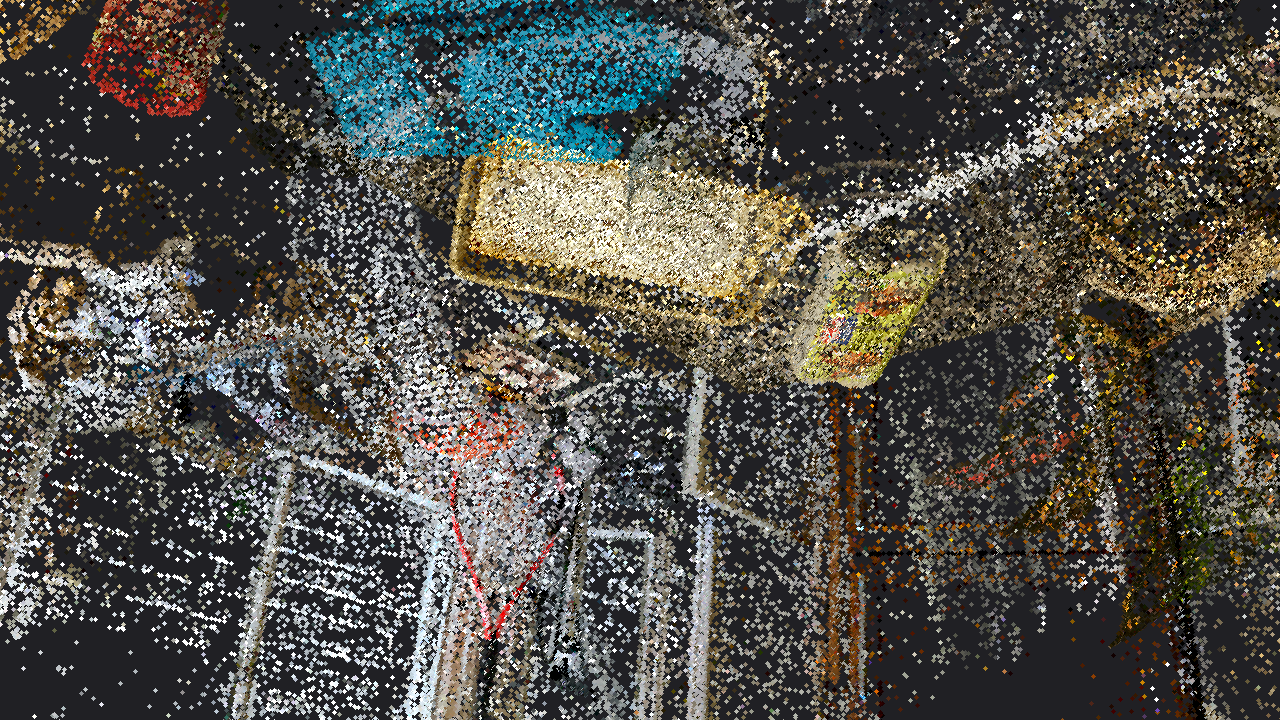
\includegraphics[width=\linewidth]{../figures/fused_frame_0060.png}
  \caption{帧 60}
\end{subfigure}
\caption{融合漫游（quality：$f_{dc}$ 颜色 + splat）}
\label{fig:fused}
\end{figure}

874{,}568 点 = 背景 + A + B/C 采样。图~\ref{fig:fused} 可见台面、窗户与三物体簇；120 帧位姿稳定。

\textbf{稀疏点云现象}：伪高斯缺 opacity/scale $\rightarrow$ splat 非照片级；legacy 版（灰度、12 万点）背景几乎不可见，quality 版显著改善。

\textbf{位姿/遮挡}：yaml 手工 Sim(3)，无 ICP；无物理阴影，交界处可能浮空/穿模——属代码级点云渲染局限，非训练失败。

%==============================================================================
\section{结论与局限}
%==============================================================================

完成 A/B/C 三路径 + counter 背景 + 融合漫游全链路。\textbf{重点贡献}：按题目要求详细阐述并实现了 Mesh$\rightarrow$伪高斯$\rightarrow$PLY 代码级统一方案，并对比 Blender 备选路径。

\textbf{结论}：A 几何纹理最优；B 最灵活但质量波动；C 便捷性与可见侧质量平衡。

\textbf{局限}：（1）融合为点云风格；（2）B/背景 loss 不完整；（3）手工位姿；（4）无定量渲染指标。未来：完整高斯参数、自动配准、Blender 附录对比。

\vspace{0.5em}
\noindent\textbf{链接}：GitHub [URL]；网盘 [URL]；WandB \url{https://wandb.ai/kryskatrina-fudan-university-school-of-management/cv-hw3}。

\section*{参考文献}
\small
[1] Huang et al., 2D Gaussian Splatting, SIGGRAPH 2024. \\
[2] Poole et al., DreamFusion, ICLR 2023. \\
[3] Qian et al., Magic123, CVPR 2024. \\
[4] Barron et al., Mip-NeRF 360, CVPR 2022.

\end{document}
